\documentclass[]{article}
\usepackage{lmodern}
\usepackage{amssymb,amsmath}
\usepackage{ifxetex,ifluatex}
\usepackage{fixltx2e} % provides \textsubscript
\ifnum 0\ifxetex 1\fi\ifluatex 1\fi=0 % if pdftex
  \usepackage[T1]{fontenc}
  \usepackage[utf8]{inputenc}
\else % if luatex or xelatex
  \ifxetex
    \usepackage{mathspec}
    \usepackage{xltxtra,xunicode}
  \else
    \usepackage{fontspec}
  \fi
  \defaultfontfeatures{Mapping=tex-text,Scale=MatchLowercase}
  \newcommand{\euro}{€}
\fi
% use upquote if available, for straight quotes in verbatim environments
\IfFileExists{upquote.sty}{\usepackage{upquote}}{}
% use microtype if available
\IfFileExists{microtype.sty}{%
\usepackage{microtype}
\UseMicrotypeSet[protrusion]{basicmath} % disable protrusion for tt fonts
}{}
\usepackage[margin=1in]{geometry}
\usepackage{longtable,booktabs}
\usepackage{graphicx}
\makeatletter
\def\maxwidth{\ifdim\Gin@nat@width>\linewidth\linewidth\else\Gin@nat@width\fi}
\def\maxheight{\ifdim\Gin@nat@height>\textheight\textheight\else\Gin@nat@height\fi}
\makeatother
% Scale images if necessary, so that they will not overflow the page
% margins by default, and it is still possible to overwrite the defaults
% using explicit options in \includegraphics[width, height, ...]{}
\setkeys{Gin}{width=\maxwidth,height=\maxheight,keepaspectratio}
\ifxetex
  \usepackage[setpagesize=false, % page size defined by xetex
              unicode=false, % unicode breaks when used with xetex
              xetex]{hyperref}
\else
  \usepackage[unicode=true]{hyperref}
\fi
\hypersetup{breaklinks=true,
            bookmarks=true,
            pdfauthor={},
            pdftitle={Supplementary Info},
            colorlinks=true,
            citecolor=blue,
            urlcolor=blue,
            linkcolor=magenta,
            pdfborder={0 0 0}}
\urlstyle{same}  % don't use monospace font for urls
\setlength{\parindent}{0pt}
\setlength{\parskip}{6pt plus 2pt minus 1pt}
\setlength{\emergencystretch}{3em}  % prevent overfull lines
\setcounter{secnumdepth}{5}

%%% Use protect on footnotes to avoid problems with footnotes in titles
\let\rmarkdownfootnote\footnote%
\def\footnote{\protect\rmarkdownfootnote}

%%% Change title format to be more compact
\usepackage{titling}

% Create subtitle command for use in maketitle
\newcommand{\subtitle}[1]{
  \posttitle{
    \begin{center}\large#1\end{center}
    }
}

\setlength{\droptitle}{-2em}

  \title{Supplementary Info: DNA methylation modules associate with incident cardiovascular disease and cumulative risk factor exposure}
    \pretitle{\vspace{\droptitle}\centering\huge}
  \posttitle{\par}
    \author{}
    \preauthor{}\postauthor{}
    \date{}
    \predate{}\postdate{}
  
\usepackage{booktabs}
\usepackage{longtable}
\usepackage{array}
\usepackage{multirow}
\usepackage[table]{xcolor}
\usepackage{wrapfig}
\usepackage{float}
\usepackage{colortbl}
\usepackage{pdflscape}
\usepackage{tabu}
\usepackage{threeparttable}
\usepackage{threeparttablex}
\usepackage[normalem]{ulem}
\usepackage{makecell}

\begin{document}

\maketitle


\newcommand{\beginsupplement}{
  \setcounter{table}{0}  
  \renewcommand{\thetable}{S\arabic{table}} 
  \setcounter{figure}{0} 
  \renewcommand{\thefigure}{S\arabic{figure}}
}

\beginsupplement

\begin{figure}[htbp]
\centering
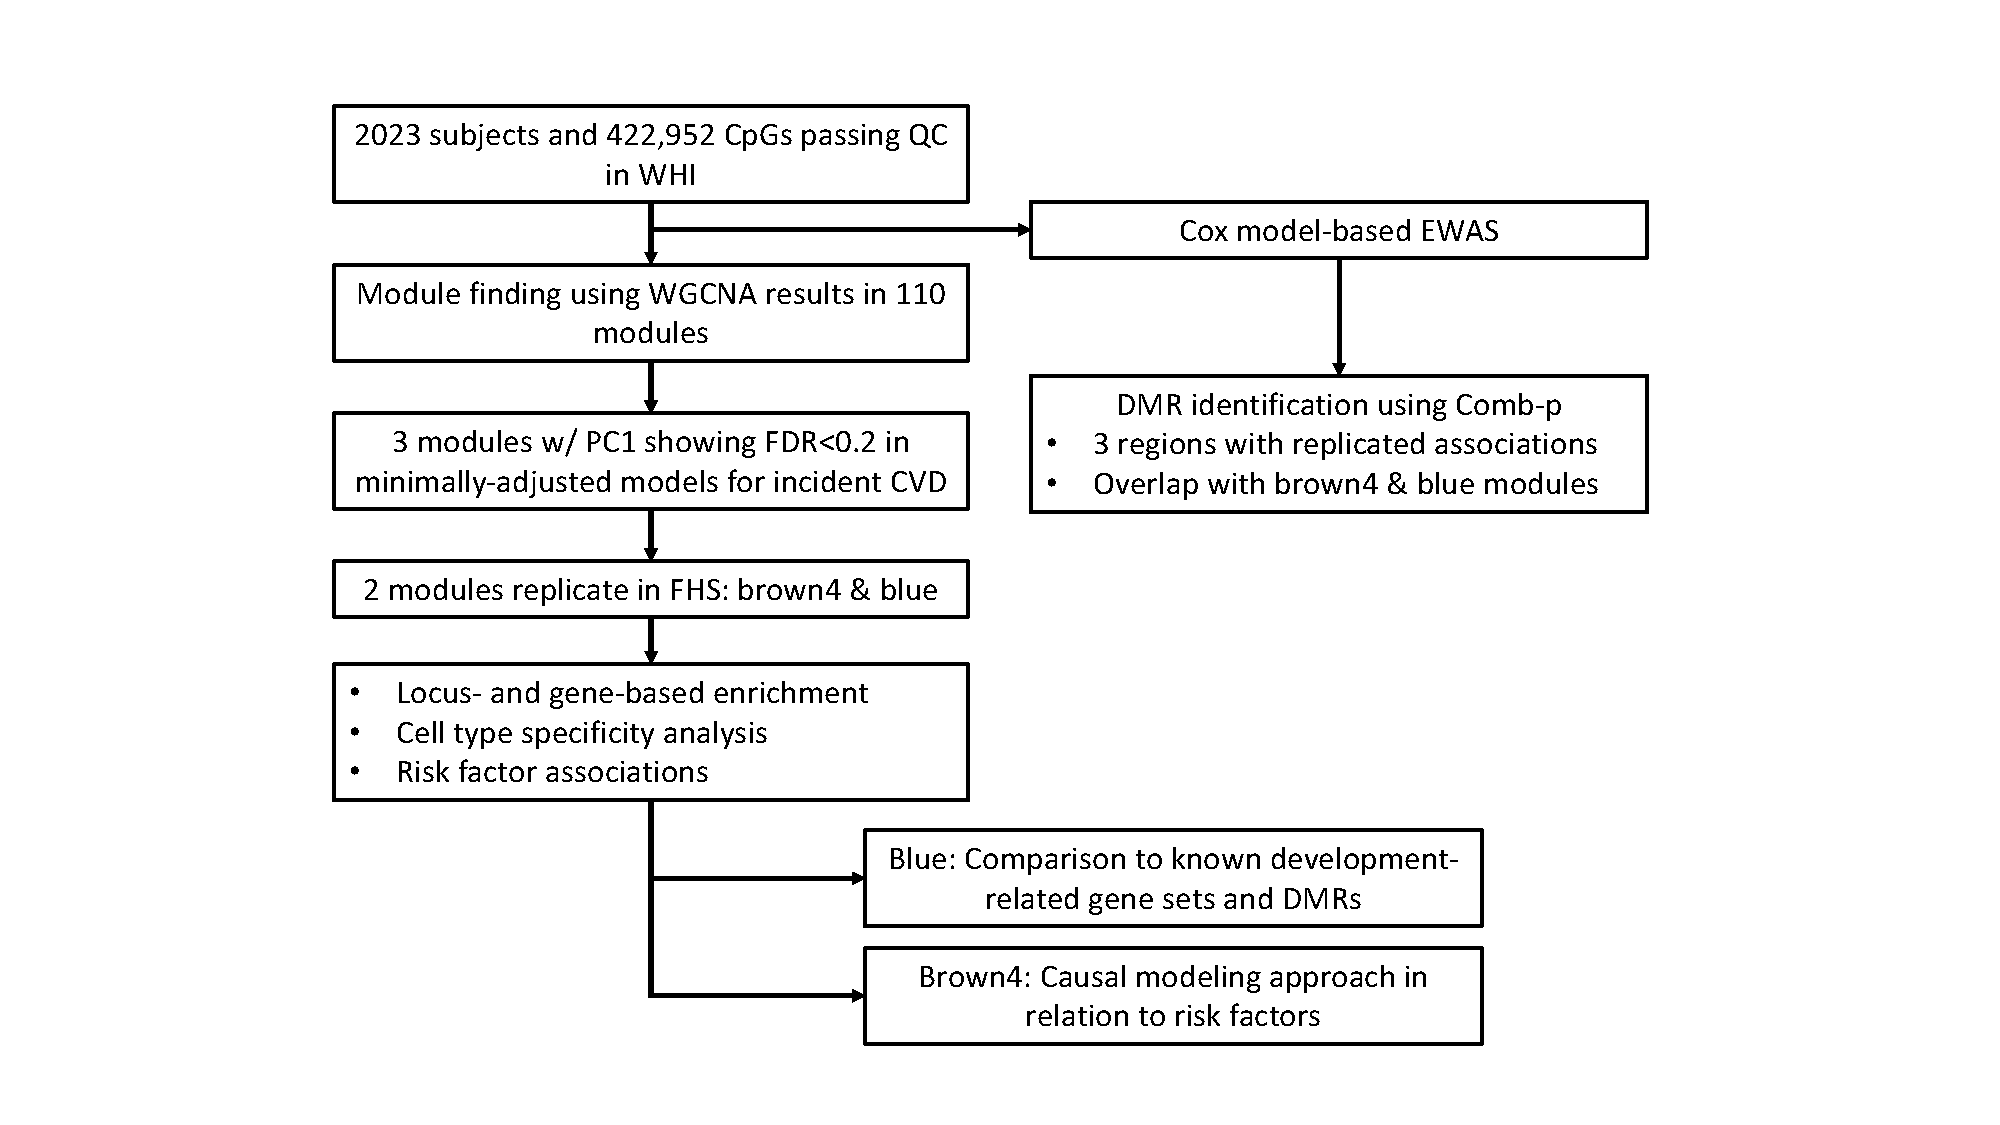
\includegraphics{../doc/module_ewas/workflow.pdf}
\caption{\label{fig:workflow}Study overview, including module- and
region-based analyses as well as follow-up.}
\end{figure}

\begin{figure}[htbp]
\centering
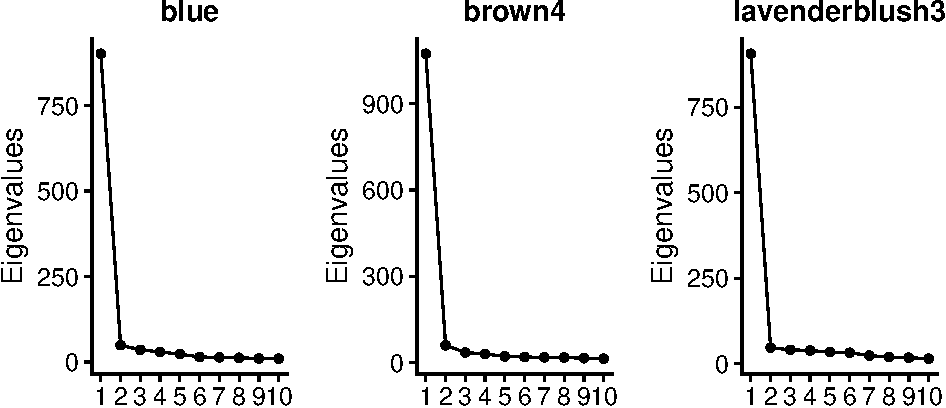
\includegraphics{../doc/module_ewas/figures/print-scree-plots-1.pdf}
\caption{\label{fig:print-scree-plots}Scree plots for PCA on the set of CpGs
corresponding to each of the top modules.}
\end{figure}

\begin{ThreePartTable}
\begin{TableNotes}
\item[1] Partially-adjusted models are adjusted for technical covariates (DNA pull batch in WHI and study center + 7 control probe PCs in FHS) and estimated cell counts. Fully-adjusted models are additionally adjusted for age, sex, smoking status and smoking pack-years.
\item[2] Mixed model contains a random intercept for each family.
\end{TableNotes}
\begin{longtable}[t]{lrrrrr}
\caption{\label{tab:module-rep-table}P-values for module associations with incident CVD in discovery and replication.}\\
\toprule
\multicolumn{1}{c}{} & \multicolumn{2}{c}{WHI (discovery)} & \multicolumn{3}{c}{FHS (replication)} \\
\cmidrule(l{2pt}r{2pt}){2-3} \cmidrule(l{2pt}r{2pt}){4-6}
Module & Partially adjusted & Fully adjusted & Partially adj. & Partially adj. (mixed) & Fully adjusted\\
\midrule
blue & 0.0002736 & 0.0500018 & 0.0000085 & 0.0000085 & 0.8189348\\
brown4 & 0.0045462 & 0.0872688 & 0.0000962 & 0.0000963 & 0.0997390\\
lavenderblush3 & 0.0050028 & 0.0210976 & 0.0202819 & 0.0202804 & 0.1580861\\
\bottomrule
\insertTableNotes
\end{longtable}
\end{ThreePartTable}

\begin{table}

\caption{\label{tab:ewas-cpgs}CpGs with FDR < 0.05 in the discovery set (Bonferroni threshold = 1.18e-7)}
\centering
\begin{tabular}[t]{lllllll}
\toprule
CpG & Chromosome & Dir. of Assoc. & P-value & Location & Annotated Gene & Replication P-value\\
\midrule
cg09155044 & chr16 & + & 6.63e-09 & TSS1500 & VKORC1 & 0.107\\
cg24434800 & chr1 & + & 5.04e-08 &  &  & 0.629\\
cg11691298 & chr2 & + & 1.1e-07 & Body & FAM59B & 0.525\\
cg02379107 & chr20 & + & 4.72e-07 & TSS1500 & KIAA1755 & 0.930\\
\bottomrule
\end{tabular}
\end{table}

\begin{figure}[htbp]
\centering
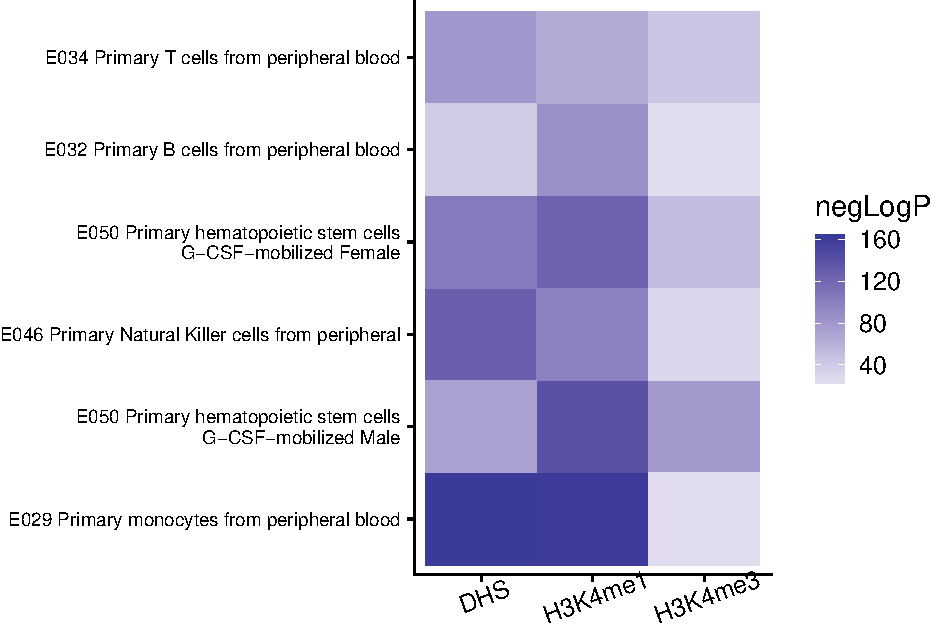
\includegraphics{../doc/module_ewas/figures/print-eforge-plots-1.pdf}
\caption{\label{fig:print-eforge-plots}eFORGE cell type-specificity plot for
the brown4 module.}
\end{figure}

\begin{figure}[htbp]
\centering
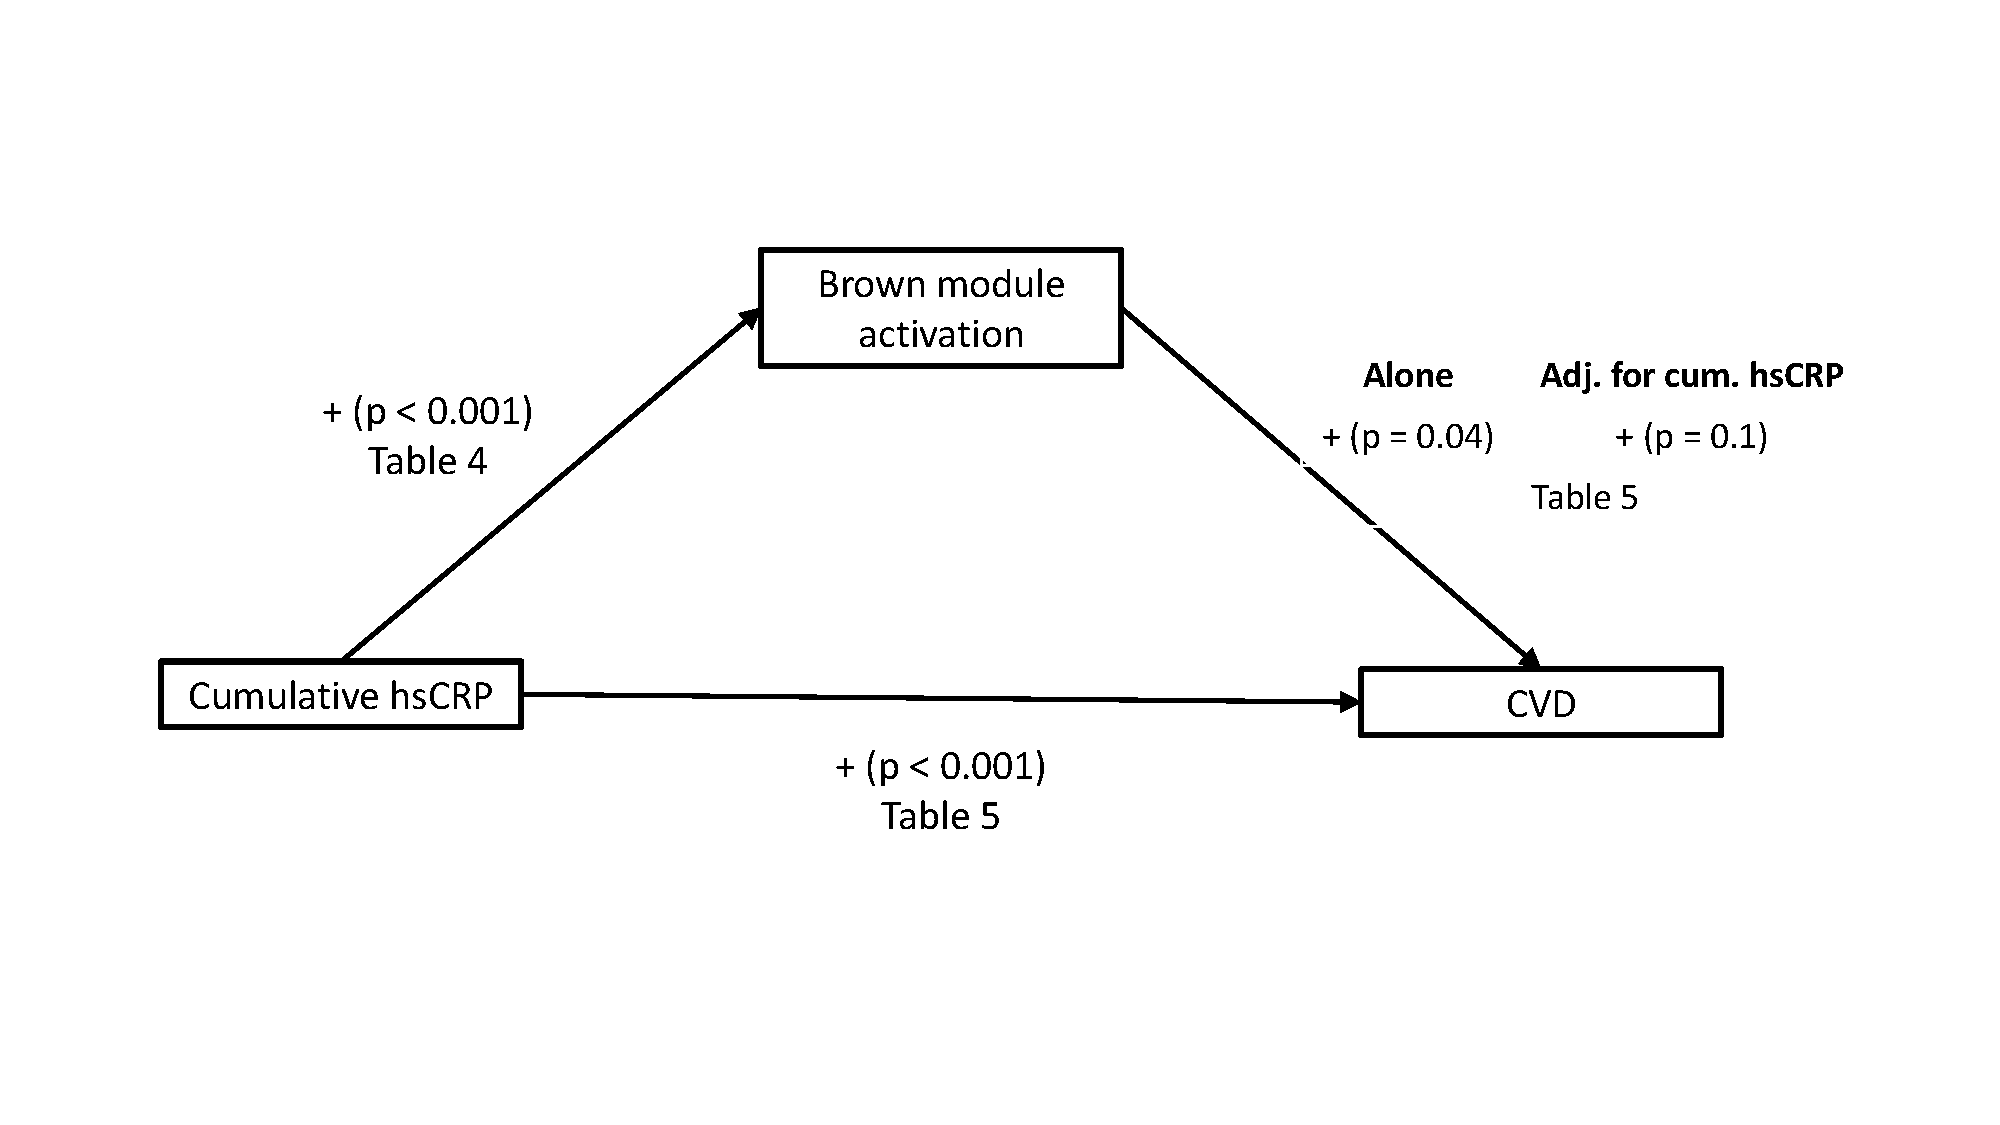
\includegraphics{../doc/module_ewas/hscrp_mediation_diagram.pdf}
\caption{\label{fig:causal-diagram-hscrp}Example diagram of cumulative risk
factor mediation by brown4 methylation module activation. Results from 4
regressions are shown: cumulative risk factor exposure to brown4
activation, cumulative risk factor exposure to incident CVD, and brown4
activation to incident CVD with and without adjustment for cumulative
risk factor exposure. Regression terms represented as: sign of
coefficient (p-value).}
\end{figure}

\end{document}
